%!TEX root = thesis.tex

\chapter{Baseline system} %TODO
\label{ch:Content1}


A system for symbol recognition was already written and is described in \cite{Kirsch}.

%!TEX root = thesis.tex
\chapter{Data, Preprocessing and Features}\label{ch:preprocessing}

\begin{wrapfigure}{r}{7cm}
  \vspace{-35pt}
  \begin{center}
    \newcommand*{\xMin}{0}%
    \newcommand*{\xMax}{6}%
    \newcommand*{\yMin}{0}%
    \newcommand*{\yMax}{6}%
    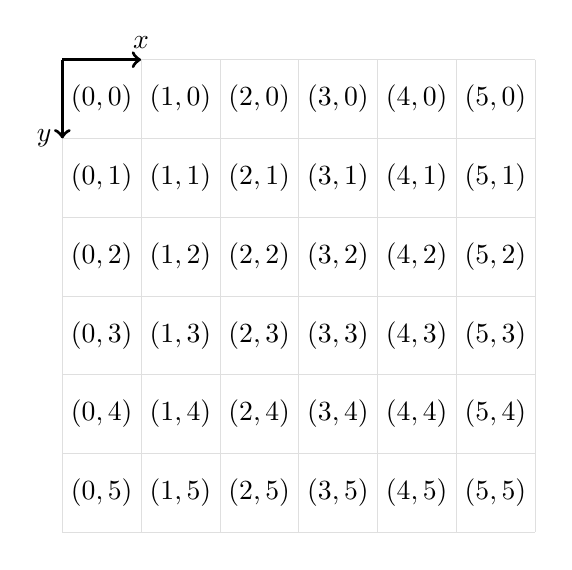
\begin{tikzpicture}[y=-1cm]
        \foreach \i in {\xMin,...,\xMax} {
            \draw [very thin,gray!25] (\i,\yMin) -- (\i,\yMax)  node [below] at (\i,\yMin) {};
        }
        \foreach \i in {\yMin,...,\yMax} {
            \draw [very thin,gray!25] (\xMin,\i) -- (\xMax,\i) node [left] at (\xMin,\i) {};
        }
        \draw[->, very thick] (0,0) -- (1,0) node[above] {$x$};
        \draw[->, very thick] (0,0) -- (0,1) node[left] {$y$};
        \foreach \x in {\xMin,...,5} {
            \foreach \y in {\yMin,...,5} {
                \node at ({\x+0.5},{\y+0.5}) {$(\x, \y)$};
            }
        }
    \end{tikzpicture}
  \end{center}
  \vspace{-20pt}
  \caption{HTML5 canvas plane. Each step is one pixel. There cannot be non-integer
           coordinates.}
  \label{fig:canvas-plane}
  \vspace{-10pt}
\end{wrapfigure}

The data that was used for all experiments was collected with
\href{http://write-math.com}{write-math.com}, a website designed solely for
this purpose. This website makes use of HTML5 canvas elements. Those elements
can be used to track fingers or a mouse coursor touching the canvas, moving
and lifting. The origin is at the upper left corner and get bigger to the right
($x$-coordinate) and to the bottom ($y$-coordinate).

The data is stored and shared in JSON format. Each handdrawing is stored as a
list of lines, where each line consists of tuples $(x, y, t)$, where $x$ and
$y$ are canvas coordinates and $t$ is a timestamp in seconds. This timestamp
gives the time in milliseconds from 1970.

The time resolution between points as well as the resolution of the image
depends on the device that was used. However, most symbols have time resolution
of about $\SI{20}{\milli\second}$ and are within a bounding box of a
$250 \text{px} \times 250 \text{px}$.

\section{Preprocessing}
\subsection{Scaling and shifting}
In many experiments the datapoints were scaled to fit into a unit square while
keeping their aspect ratio. Afterwards, the points were shifted to the
$(0, 1) \times (0, 1)$ unit square. The algorithm is given in pseudocode on
\cpageref{alg:scale-and-shift}. It was shown in \cite{Kirsch,Huang09} that
this kind of preprocessing boosts classification accuracy significantly.

\section{Features}
A number of different features have been suggested so far for on-line handwriting
recognition. They can be grouped into local features and global features.
Local features apply to a given point on the drawing plane and sometimes even
only to point on the drawn curve whereas global features apply to a complete
line or even the complete image.

\subsection{Local features}
\begin{itemize}
    \item Curvature\cite{Manke95}
    \item Speed\cite{Huang09}
    \item Binary pen pressure\cite{Kosmala98,Kosmala11}
    \item Direction\cite{Manke95,Huang06}
    \item Bitmap-environment\cite{Manke95}
\end{itemize}

\cite{Kosmala98,Kosmala11} suggest that speed is a bad feature, because it \enquote{highly inconsistent}.

\subsection{Global features}
\begin{itemize}
    \item Re-curvature\cite{Huang06} (TODO: Explain (all))
    \item Center point\cite{Huang06}
    \item Stroke length\cite{Huang06}
    \item Number of strokes\cite{Huang09}
    \item Pseudo-Zernike Features (TODO: Really global? What is it?)\cite{Khotanzad}
    \item Shadow Code Features\cite{Khotanzad}
\end{itemize}

\chapter{Artificial Neural Nets}\label{ch:ANNs}

\Glspl{ANN} are models for classification that were inspired by the brain.
They consist of artificial neurons and have a lot of different subtypes like
Feed Forward Neural Nets.

%!TEX root = thesis.tex
\section{Artificial neurons}\label{sec:artificial-neurons}
%% ===========================

Artificial neurons are inspired by biological neurons. Signals are send within 
the cell by charged particles, so called \textit{ions}. But before a biological
neuron sends a signal, a threshold charge has to be reached at the axon
hillock. This threshold charge is called \textit{action potential}. The action
potential can be reached by multiple factors, but the one I want to focus on
are charges send by other neurons. Depending on where the other axon terminals
are located and how long the distance to the axon hillock is, the signal contributes
more or less to reaching the action potential. After that, it simply sends a
signal.

\begin{figure}[ht]
    \centering
    \subfloat[Biological Neuron]{
        \includegraphics*[width=0.48\linewidth, keepaspectratio]{figures/biological-neuron.jpg} 
        \label{fig:biological-neuron}
    }%
    \subfloat[Artificial Neuron]{
        \resizebox{0.45\linewidth}{!}{\input{figures/artificial-neuron.tex}}
        \label{fig:artificial-neuron}
    }%
    \label{fig:artificial-and-biological-neuron}
    \caption{Both neurons receive weighted input, apply a function to that and give output}
\end{figure}

Artificial neurons are similar. They receive at least one input and give at
least one output. Those inputs might get weighted as well as the output.

The neurons apply a function to the sum of all weighted inputs. This function
is also called \textit{activation function}.

An artificial neuron using the unit step function (see \cref{f:unitstep}) is called
a \textit{perceptron}.


The artificial neuron sums all weighted inputs $x_i \cdot w_i$ up
             and applies its activation function $f$ to it.
%!TEX root = thesis.tex
\section{Multilayer Perceptron}\label{ch:Content2:sec:Section2}

\Glspl{MLP} are neural nets whichs neurons are structured in layers.
Each layer is fully connected with the next layer, but there are no other
connections between neurons.

\begin{figure}[ht]
    \centering
    %!TEX root = thesis.tex
\section{Multilayer Perceptron}\label{ch:Content2:sec:Section2}

\Glspl{MLP} are neural nets whichs neurons are structured in layers.
Each layer is fully connected with the next layer, but there are no other
connections between neurons.

\begin{figure}[ht]
    \centering
    %!TEX root = thesis.tex
\section{Multilayer Perceptron}\label{ch:Content2:sec:Section2}

\Glspl{MLP} are neural nets whichs neurons are structured in layers.
Each layer is fully connected with the next layer, but there are no other
connections between neurons.

\begin{figure}[ht]
    \centering
    \input{figures/feedforward.tex}
    \caption{Feedforward artificial neural network}
    \label{fig:feedforward}
\end{figure}

The red neurons in \cref{fig:feedforward} are input neurons, the green ones are
hidden neurons and the blue one is an output node. The gray neurons are bias neurons.
Bias neurons have a fixed output of $1$.

Usually, you have as many output neurons as you have classes. So in the case of
symbol recognition that would be about $\si{1076}$ neurons.

The number of input neurons is equal to the number of features.

\section{Notation}
Let $n_i$ be the number of neurons in the $i$-th layer and $\layernumber$ be the
number of layers of the \gls{MLP}.

Two neighboring layers of neurons are fully connected and have weights between
two layers. This means you can store those weights in form of matrices.
So the weights between layer $i$ and layer $i+1$ are

\[W_i = \begin{pmatrix}
    w_{1,1} & w_{1,2} & \dots & w_{1,n_{i+1}}\\
    w_{2,1} & w_{2,2} & \dots & w_{2,n_{i+1}}\\
    w_{3,1} & w_{3,2} & \dots & w_{3,n_{i+1}}\\
    \vdots  &         & \ddots& \vdots \\
    w_{n_{i},1} & w_{n_{i},2} & \dots & w_{n_{i},n_{i+1}}
\end{pmatrix}\]

Let $w_{ij}^{(k)}$ be the value $w_{ij}$ in $W_k$. So it is the weight of the
between neuron $i$ in layer $k$ and neuron $j$ in layer $k+1$.

So $W_i \in \mdr^{n_i \times n_{i+1}}$ is the matrix denoting the weights between layer
$i$ and layer $i+1$.

The unweighted output vector of layer $i$ is denoted by $x_i \in \mdr^{1 \times n_i}$;
the weighted output vector by $\net_i \in \mdr^{1 \times n_i}$. Instead of $x_1$ I
will write $x$.
The output of the \gls{MLP} for the input $x$ is denoted by $o_x:= x_n$.

In principle each neuron might have a different activation function, but in
practice each neuron in one layer has the same activation function. However,
activation functions might differ from layer to layer. This is the reason why
I denote the activation function of layer $i$ by $\varphi_i$. Although $\varphi_i$
is defined for single neurons, I will in the following apply it to vectors. In
its meant to be applied pointwise.

The activation function is a function 

\[\varphi_i: \mdr \rightarrow \mdr \]

but because of the short-notation it can be applied pointwise to all neurons
of layer $i$ it is also a function

\[\varphi_i: \mdr^{n_{i}} \rightarrow \mdr^{n_{i}}\]

\section{Evaluation}
Let $x_1 \in \mdr^{1 \times n_1}$ be an unweighted output of layer $1$. So it's
simply the input of our neural net with $n_1$ features.

Given $x_1$ one can easily compute the weighted input for layer $2$:

\[
\begin{array}{@{}c@{\;}c@{\;}c@{\;}c@{\;}c@{}}
x_1 & \cdot & W_{1} & = & \net_1 \\
\vin && \vin && \vin \\
\mathbb{R}^{1\times n_1} && \mathbb{R}^{n_1\times n_2} && \mathbb{R}^{1\times n_2}
\end{array}
\]

After that, you can apply the activation function $\varphi_{i+1}$ pointwise
to $\net_i$. %TODO: Is that really called "pointwise" application?

So the output vector $x_3$ of a 3-layer (input, hidden, output) neural net can be
computed by

\[x_3 = \varphi_3(\varphi_2(x_1 \cdot W_{1}) \cdot W_{2})\]

The output of a general \gls{MLP} can be computed by

\begin{align*}
    \Phi(x, n) &: \mdr^{n_1} \rightarrow \mdr^{n_n}\\
    \Phi(x_1, 2) &:= \varphi_{2}(x_1 \cdot W_{1})\\
    \Phi(x, n) &:= \varphi_{n} \left (\Phi(x, n-1) \cdot W_{n-1} \right)\\
    \Phi(x, n)^{(p)} &= \varphi_n \left ( \sum_{i=1}^{n_{n-1}} \Phi(x, n-1)^{(i)} \cdot w_{ip}^{(n-1)} \right )
\end{align*}

It follows: $x_i(x_1) = \Phi(x_1, i)$.

\section{Supervised Training with Backpropagation}\label{sec:training}
The backpropagation algorithm is a supervised algorithm for training
\glspl{MLP}. This means the trainigset $T$ consists of tuples $(x, t_x)$
where $x$ is input and $t_x$ is the desired output.

To evaluate how good the current \gls{MLP} is, an error function can be defined:

\begin{align*}
    E: \mdr^{n_1 \times n_2} \times \mdr^{n_2 \times n_3} \times \dots \times \mdr^{n_{\layernumber-1, \layernumber}} \rightarrow \mdr_{\geq 0}\\
    E_T(W) = \frac{1}{2} \sum_{(x, t_x) \in T} \sum_{p = 1}^{n_\layernumber} \left (t_{x}^{(p)} - o_{x}^{(p)} \right )^2
\end{align*}

This function is isomorphic to 

\[E: \mdr^{\sum_{i=2}^\layernumber n_{i-1} \cdot n_{i}} \rightarrow \mdr_{\geq 0}\]

This error should be minimized. As the error is the sum of non-negative values,
we will get a lower error by minimizing the error for a single training example.
However, note that those minimizations are not independant. This means, we could
get trapped in a local minimum.

The idea is to \enquote{go} into the direction in which the error $E$ decreases
most. This is the gradient and the process is thus called \textit{gradient descent}.

At this point we need to decide how far we want to go. If we make too big steps
in the direction of the gradient, we might overshoot. If we make too small steps,
the algorithm will take too long to get to the minimum. As reducing the error
is basically learning the number is called learning rate $\eta \in \mdr_{> 0}$.

So the algorithm is

\begin{algorithm}[h]
    \begin{algorithmic}
        \Function{backpropagate}{$T$, $W$}
            \While{True}
                \ForAll{$(x, t_x) \in T$}
                    \ForAll{node $i$}
                        \ForAll{nodes $j$ following $i$}
                            \State $\displaystyle w_{ijk} \gets w_{ijk} - \eta \frac{\partial E_{\Set{x}}}{\partial w_{ijk}} (W)$
                        \EndFor
                    \EndFor
                \EndFor
            \EndWhile
        \EndFunction
    \end{algorithmic}
\caption{Backpropagate}
\label{alg:backpropagate}
\end{algorithm}

Computing the partial derivatives $\frac{\partial E_{\Set{x}}}{\partial w_{ijk}}$
is not a trivial task. To do that, we have to take a closer look at the
error function:

% \begin{align}
%     \frac{\partial E_{\Set{x}}}{\partial w_{ijk}}
%     &= \frac{\partial}{\partial w_{ijk}} \frac{1}{2} \sum_{(x, t_x) \in T} \sum_{p = 1}^{|n_\layernumber|} \left (t_{x}^{(p)} - o_{x}^{(p)} \right )^2\\
%     &= \frac{1}{2} \sum_{(x, t_x) \in T} \sum_{p = 1}^{|n_\layernumber|} \frac{\partial}{\partial w_{ijk}} \left (t_{x}^{(p)} - o_{x}^{(p)} \right )^2\\
%     &= \frac{1}{2} \sum_{(x, t_x) \in T} \sum_{p = 1}^{|n_\layernumber|} 2 \left (t_{x}^{(p)} - o_{x}^{(p)} \right ) \cdot \frac{\partial}{\partial w_{ijk}} \left (t_{x}^{(p)} - o_{x}^{(p)} \right )\\
%     &= - \sum_{(x, t_x) \in T} \sum_{p = 1}^{|n_\layernumber|} \left (t_{x}^{(p)} - o_{x}^{(p)} \right ) \cdot \frac{\partial}{\partial w_{ijk}}
%     \left (
%         \varphi_{\layernumber}(
%             \underbrace{\Phi_W(x, \layernumber-1)}_{\stackrel{\vin}{\mdr^{1 \times n_{\layernumber-1}}}}
%             \cdot 
%             \underbrace{W_{\layernumber-1}}_{\stackrel{\vin}{\mdr^{n_{\layernumber-1}, n_\layernumber}}}
%         )^{(p)}
%     \right)
% \end{align}

% The function $\varphi_{\layernumber}$ is applied component wise and we are
% only interested in the result of the $p$-th element of the result vector. 

% As $p$ is bound in the inner sum, we can ignore that we have vectors
% but instead think of it as a function
% $\varphi_l: \mdr \rightarrow \mdr$:

% \begin{align}
%     \frac{\partial}{\partial w_{ijk}}
%         \varphi_{\layernumber} \left (
%             \sum_{i=1}^{n_{\layernumber-1}} \Phi(x, \layernumber-1)^{(i)}
%             \cdot 
%             W_{\layernumber-1}^{(i,p)}
%         \right )
%     &= \varphi_{\layernumber}' \left (
%             \sum_{i=1}^{n_{\layernumber-1}} x_{\layernumber-1}
%             \cdot 
%             W_{\layernumber-1}^{(i,p)}
%        \right )
%        \cdot
%        x_{\layernumber-1} % TODO!!!
%     \\
%     &= \varphi_{\layernumber}' (\net_{\layernumber-1}^{(p)})
%        \cdot
%        x_{\layernumber-1} % TODO!!!
% \end{align}


% ------

Another approach:

\begin{align}
    E_x(W) &= \frac{1}{2} \sum_{p=1}^{n_\layernumber} \left ( t_x^{(p)} -o_x^{(p)} \right )^2\\
    o_x^{(p)} &= \Phi(x, \layernumber)^{(p)} \\
              &= \varphi_{\layernumber} \big (\Phi(x, \layernumber-1) \cdot W_{\layernumber-1} \big)^{(p)}\\
              &= \varphi_{\layernumber} \big (
                  \underbrace{
                      \sum_{i=1}^{n_{\layernumber-1}} \Phi(x, \layernumber-1)^{(i)} \cdot w_{ip}^{(\layernumber-1)}
                  }_{\net_{\layernumber-1}^{(p)}} \big)\\
    \frac{\partial E_x}{\partial w_{ij}^{(k)}} &= \frac{\partial E_x}{\partial \net_k^{(j)}} \frac{\partial \net_k^{(j)}}{\partial w_{ij}^{(k)}}\\
    &= \frac{\partial E_x}{\partial \net_k^{(j)}} \frac{\sum_{i=1}^{n_{k}} \Phi(x, k)^{(i)} \cdot w_{ij}^{(k)}}{\partial w_{ij}^{(k)}}\\
    &= \frac{\partial E_x}{\partial \net_k^{(j)}} \Phi(x, k)^{(i)}
\end{align}

Suppose $k = \layernumber - 1$ (weights to the output layer). Then:

\begin{align}
    \frac{\partial E_x}{\partial w_{ij}^{(\layernumber-1)}} &= \frac{\partial E_x}{\partial \net_{\layernumber-1}^{(j)}} \Phi(x, \layernumber-1)^{(i)}\\
    &= \frac{\frac{1}{2} \sum_{p=1}^{n_\layernumber} \left ( t_x^{(p)} -o_x^{(p)} \right )^2}{\partial \net_{\layernumber-1}^{(j)}} \Phi(x, \layernumber-1)^{(i)}\\
    &= \frac{\frac{1}{2} \sum_{p=1}^{n_\layernumber} \left ( t_x^{(p)} -\varphi_{\layernumber}(\net_{\layernumber-1})^{(p)} \right )^2}{\partial \net_{\layernumber-1}^{(j)}} \Phi(x, \layernumber-1)^{(i)}\\ % I can put this to the top
    &= \left (
            (t_x^{(j)} - \varphi_{\layernumber}(\net_{\layernumber-1}^{(j)})) \cdot (- \varphi_{\layernumber}'(\net_{\layernumber-1}^{(j)}))
       \right ) \Phi(x, \layernumber-1)^{(i)}
\end{align}

%If you further assume that $\varphi_{}$

Suppose $k = \layernumber - 2$ (last hidden layer). Then:

\begin{align}
    \frac{\partial E_x}{\partial w_{ij}^{(\layernumber-2)}} &= \frac{\frac{1}{2} \sum_{p=1}^{n_\layernumber} \left ( t_x^{(p)} -\varphi_{\layernumber}(\net_{\layernumber-1})^{(p)} \right )^2}{\partial \net_{\layernumber-2}^{(j)}} \Phi(x, \layernumber-2)^{(i)}\\
    &= \frac{\frac{1}{2} \sum_{p=1}^{n_\layernumber} \left ( t_x^{(p)} -\varphi_{\layernumber}(\sum_{i=1}^{n_{\layernumber-1}} (
        \varphi_{\layernumber-1} \big (\varphi_{\layernumber-2}(\net_{\layernumber-2}^{(j)}) \big)
    )^{(i)} \cdot w_{ip}^{(\layernumber-1)})^{(p)} \right )^2}{\partial \net_{\layernumber-2}^{(j)}} \Phi(x, \layernumber-2)^{(i)}\\
\end{align}
    \caption{Feedforward artificial neural network}
    \label{fig:feedforward}
\end{figure}

The red neurons in \cref{fig:feedforward} are input neurons, the green ones are
hidden neurons and the blue one is an output node. The gray neurons are bias neurons.
Bias neurons have a fixed output of $1$.

Usually, you have as many output neurons as you have classes. So in the case of
symbol recognition that would be about $\si{1076}$ neurons.

The number of input neurons is equal to the number of features.

\section{Notation}
Let $n_i$ be the number of neurons in the $i$-th layer and $\layernumber$ be the
number of layers of the \gls{MLP}.

Two neighboring layers of neurons are fully connected and have weights between
two layers. This means you can store those weights in form of matrices.
So the weights between layer $i$ and layer $i+1$ are

\[W_i = \begin{pmatrix}
    w_{1,1} & w_{1,2} & \dots & w_{1,n_{i+1}}\\
    w_{2,1} & w_{2,2} & \dots & w_{2,n_{i+1}}\\
    w_{3,1} & w_{3,2} & \dots & w_{3,n_{i+1}}\\
    \vdots  &         & \ddots& \vdots \\
    w_{n_{i},1} & w_{n_{i},2} & \dots & w_{n_{i},n_{i+1}}
\end{pmatrix}\]

Let $w_{ij}^{(k)}$ be the value $w_{ij}$ in $W_k$. So it is the weight of the
between neuron $i$ in layer $k$ and neuron $j$ in layer $k+1$.

So $W_i \in \mdr^{n_i \times n_{i+1}}$ is the matrix denoting the weights between layer
$i$ and layer $i+1$.

The unweighted output vector of layer $i$ is denoted by $x_i \in \mdr^{1 \times n_i}$;
the weighted output vector by $\net_i \in \mdr^{1 \times n_i}$. Instead of $x_1$ I
will write $x$.
The output of the \gls{MLP} for the input $x$ is denoted by $o_x:= x_n$.

In principle each neuron might have a different activation function, but in
practice each neuron in one layer has the same activation function. However,
activation functions might differ from layer to layer. This is the reason why
I denote the activation function of layer $i$ by $\varphi_i$. Although $\varphi_i$
is defined for single neurons, I will in the following apply it to vectors. In
its meant to be applied pointwise.

The activation function is a function 

\[\varphi_i: \mdr \rightarrow \mdr \]

but because of the short-notation it can be applied pointwise to all neurons
of layer $i$ it is also a function

\[\varphi_i: \mdr^{n_{i}} \rightarrow \mdr^{n_{i}}\]

\section{Evaluation}
Let $x_1 \in \mdr^{1 \times n_1}$ be an unweighted output of layer $1$. So it's
simply the input of our neural net with $n_1$ features.

Given $x_1$ one can easily compute the weighted input for layer $2$:

\[
\begin{array}{@{}c@{\;}c@{\;}c@{\;}c@{\;}c@{}}
x_1 & \cdot & W_{1} & = & \net_1 \\
\vin && \vin && \vin \\
\mathbb{R}^{1\times n_1} && \mathbb{R}^{n_1\times n_2} && \mathbb{R}^{1\times n_2}
\end{array}
\]

After that, you can apply the activation function $\varphi_{i+1}$ pointwise
to $\net_i$. %TODO: Is that really called "pointwise" application?

So the output vector $x_3$ of a 3-layer (input, hidden, output) neural net can be
computed by

\[x_3 = \varphi_3(\varphi_2(x_1 \cdot W_{1}) \cdot W_{2})\]

The output of a general \gls{MLP} can be computed by

\begin{align*}
    \Phi(x, n) &: \mdr^{n_1} \rightarrow \mdr^{n_n}\\
    \Phi(x_1, 2) &:= \varphi_{2}(x_1 \cdot W_{1})\\
    \Phi(x, n) &:= \varphi_{n} \left (\Phi(x, n-1) \cdot W_{n-1} \right)\\
    \Phi(x, n)^{(p)} &= \varphi_n \left ( \sum_{i=1}^{n_{n-1}} \Phi(x, n-1)^{(i)} \cdot w_{ip}^{(n-1)} \right )
\end{align*}

It follows: $x_i(x_1) = \Phi(x_1, i)$.

\section{Supervised Training with Backpropagation}\label{sec:training}
The backpropagation algorithm is a supervised algorithm for training
\glspl{MLP}. This means the trainigset $T$ consists of tuples $(x, t_x)$
where $x$ is input and $t_x$ is the desired output.

To evaluate how good the current \gls{MLP} is, an error function can be defined:

\begin{align*}
    E: \mdr^{n_1 \times n_2} \times \mdr^{n_2 \times n_3} \times \dots \times \mdr^{n_{\layernumber-1, \layernumber}} \rightarrow \mdr_{\geq 0}\\
    E_T(W) = \frac{1}{2} \sum_{(x, t_x) \in T} \sum_{p = 1}^{n_\layernumber} \left (t_{x}^{(p)} - o_{x}^{(p)} \right )^2
\end{align*}

This function is isomorphic to 

\[E: \mdr^{\sum_{i=2}^\layernumber n_{i-1} \cdot n_{i}} \rightarrow \mdr_{\geq 0}\]

This error should be minimized. As the error is the sum of non-negative values,
we will get a lower error by minimizing the error for a single training example.
However, note that those minimizations are not independant. This means, we could
get trapped in a local minimum.

The idea is to \enquote{go} into the direction in which the error $E$ decreases
most. This is the gradient and the process is thus called \textit{gradient descent}.

At this point we need to decide how far we want to go. If we make too big steps
in the direction of the gradient, we might overshoot. If we make too small steps,
the algorithm will take too long to get to the minimum. As reducing the error
is basically learning the number is called learning rate $\eta \in \mdr_{> 0}$.

So the algorithm is

\begin{algorithm}[h]
    \begin{algorithmic}
        \Function{backpropagate}{$T$, $W$}
            \While{True}
                \ForAll{$(x, t_x) \in T$}
                    \ForAll{node $i$}
                        \ForAll{nodes $j$ following $i$}
                            \State $\displaystyle w_{ijk} \gets w_{ijk} - \eta \frac{\partial E_{\Set{x}}}{\partial w_{ijk}} (W)$
                        \EndFor
                    \EndFor
                \EndFor
            \EndWhile
        \EndFunction
    \end{algorithmic}
\caption{Backpropagate}
\label{alg:backpropagate}
\end{algorithm}

Computing the partial derivatives $\frac{\partial E_{\Set{x}}}{\partial w_{ijk}}$
is not a trivial task. To do that, we have to take a closer look at the
error function:

% \begin{align}
%     \frac{\partial E_{\Set{x}}}{\partial w_{ijk}}
%     &= \frac{\partial}{\partial w_{ijk}} \frac{1}{2} \sum_{(x, t_x) \in T} \sum_{p = 1}^{|n_\layernumber|} \left (t_{x}^{(p)} - o_{x}^{(p)} \right )^2\\
%     &= \frac{1}{2} \sum_{(x, t_x) \in T} \sum_{p = 1}^{|n_\layernumber|} \frac{\partial}{\partial w_{ijk}} \left (t_{x}^{(p)} - o_{x}^{(p)} \right )^2\\
%     &= \frac{1}{2} \sum_{(x, t_x) \in T} \sum_{p = 1}^{|n_\layernumber|} 2 \left (t_{x}^{(p)} - o_{x}^{(p)} \right ) \cdot \frac{\partial}{\partial w_{ijk}} \left (t_{x}^{(p)} - o_{x}^{(p)} \right )\\
%     &= - \sum_{(x, t_x) \in T} \sum_{p = 1}^{|n_\layernumber|} \left (t_{x}^{(p)} - o_{x}^{(p)} \right ) \cdot \frac{\partial}{\partial w_{ijk}}
%     \left (
%         \varphi_{\layernumber}(
%             \underbrace{\Phi_W(x, \layernumber-1)}_{\stackrel{\vin}{\mdr^{1 \times n_{\layernumber-1}}}}
%             \cdot 
%             \underbrace{W_{\layernumber-1}}_{\stackrel{\vin}{\mdr^{n_{\layernumber-1}, n_\layernumber}}}
%         )^{(p)}
%     \right)
% \end{align}

% The function $\varphi_{\layernumber}$ is applied component wise and we are
% only interested in the result of the $p$-th element of the result vector. 

% As $p$ is bound in the inner sum, we can ignore that we have vectors
% but instead think of it as a function
% $\varphi_l: \mdr \rightarrow \mdr$:

% \begin{align}
%     \frac{\partial}{\partial w_{ijk}}
%         \varphi_{\layernumber} \left (
%             \sum_{i=1}^{n_{\layernumber-1}} \Phi(x, \layernumber-1)^{(i)}
%             \cdot 
%             W_{\layernumber-1}^{(i,p)}
%         \right )
%     &= \varphi_{\layernumber}' \left (
%             \sum_{i=1}^{n_{\layernumber-1}} x_{\layernumber-1}
%             \cdot 
%             W_{\layernumber-1}^{(i,p)}
%        \right )
%        \cdot
%        x_{\layernumber-1} % TODO!!!
%     \\
%     &= \varphi_{\layernumber}' (\net_{\layernumber-1}^{(p)})
%        \cdot
%        x_{\layernumber-1} % TODO!!!
% \end{align}


% ------

Another approach:

\begin{align}
    E_x(W) &= \frac{1}{2} \sum_{p=1}^{n_\layernumber} \left ( t_x^{(p)} -o_x^{(p)} \right )^2\\
    o_x^{(p)} &= \Phi(x, \layernumber)^{(p)} \\
              &= \varphi_{\layernumber} \big (\Phi(x, \layernumber-1) \cdot W_{\layernumber-1} \big)^{(p)}\\
              &= \varphi_{\layernumber} \big (
                  \underbrace{
                      \sum_{i=1}^{n_{\layernumber-1}} \Phi(x, \layernumber-1)^{(i)} \cdot w_{ip}^{(\layernumber-1)}
                  }_{\net_{\layernumber-1}^{(p)}} \big)\\
    \frac{\partial E_x}{\partial w_{ij}^{(k)}} &= \frac{\partial E_x}{\partial \net_k^{(j)}} \frac{\partial \net_k^{(j)}}{\partial w_{ij}^{(k)}}\\
    &= \frac{\partial E_x}{\partial \net_k^{(j)}} \frac{\sum_{i=1}^{n_{k}} \Phi(x, k)^{(i)} \cdot w_{ij}^{(k)}}{\partial w_{ij}^{(k)}}\\
    &= \frac{\partial E_x}{\partial \net_k^{(j)}} \Phi(x, k)^{(i)}
\end{align}

Suppose $k = \layernumber - 1$ (weights to the output layer). Then:

\begin{align}
    \frac{\partial E_x}{\partial w_{ij}^{(\layernumber-1)}} &= \frac{\partial E_x}{\partial \net_{\layernumber-1}^{(j)}} \Phi(x, \layernumber-1)^{(i)}\\
    &= \frac{\frac{1}{2} \sum_{p=1}^{n_\layernumber} \left ( t_x^{(p)} -o_x^{(p)} \right )^2}{\partial \net_{\layernumber-1}^{(j)}} \Phi(x, \layernumber-1)^{(i)}\\
    &= \frac{\frac{1}{2} \sum_{p=1}^{n_\layernumber} \left ( t_x^{(p)} -\varphi_{\layernumber}(\net_{\layernumber-1})^{(p)} \right )^2}{\partial \net_{\layernumber-1}^{(j)}} \Phi(x, \layernumber-1)^{(i)}\\ % I can put this to the top
    &= \left (
            (t_x^{(j)} - \varphi_{\layernumber}(\net_{\layernumber-1}^{(j)})) \cdot (- \varphi_{\layernumber}'(\net_{\layernumber-1}^{(j)}))
       \right ) \Phi(x, \layernumber-1)^{(i)}
\end{align}

%If you further assume that $\varphi_{}$

Suppose $k = \layernumber - 2$ (last hidden layer). Then:

\begin{align}
    \frac{\partial E_x}{\partial w_{ij}^{(\layernumber-2)}} &= \frac{\frac{1}{2} \sum_{p=1}^{n_\layernumber} \left ( t_x^{(p)} -\varphi_{\layernumber}(\net_{\layernumber-1})^{(p)} \right )^2}{\partial \net_{\layernumber-2}^{(j)}} \Phi(x, \layernumber-2)^{(i)}\\
    &= \frac{\frac{1}{2} \sum_{p=1}^{n_\layernumber} \left ( t_x^{(p)} -\varphi_{\layernumber}(\sum_{i=1}^{n_{\layernumber-1}} (
        \varphi_{\layernumber-1} \big (\varphi_{\layernumber-2}(\net_{\layernumber-2}^{(j)}) \big)
    )^{(i)} \cdot w_{ip}^{(\layernumber-1)})^{(p)} \right )^2}{\partial \net_{\layernumber-2}^{(j)}} \Phi(x, \layernumber-2)^{(i)}\\
\end{align}
    \caption{Feedforward artificial neural network}
    \label{fig:feedforward}
\end{figure}

The red neurons in \cref{fig:feedforward} are input neurons, the green ones are
hidden neurons and the blue one is an output node. The gray neurons are bias neurons.
Bias neurons have a fixed output of $1$.

Usually, you have as many output neurons as you have classes. So in the case of
symbol recognition that would be about $\si{1076}$ neurons.

The number of input neurons is equal to the number of features.

\section{Notation}
Let $n_i$ be the number of neurons in the $i$-th layer and $\layernumber$ be the
number of layers of the \gls{MLP}.

Two neighboring layers of neurons are fully connected and have weights between
two layers. This means you can store those weights in form of matrices.
So the weights between layer $i$ and layer $i+1$ are

\[W_i = \begin{pmatrix}
    w_{1,1} & w_{1,2} & \dots & w_{1,n_{i+1}}\\
    w_{2,1} & w_{2,2} & \dots & w_{2,n_{i+1}}\\
    w_{3,1} & w_{3,2} & \dots & w_{3,n_{i+1}}\\
    \vdots  &         & \ddots& \vdots \\
    w_{n_{i},1} & w_{n_{i},2} & \dots & w_{n_{i},n_{i+1}}
\end{pmatrix}\]

Let $w_{ij}^{(k)}$ be the value $w_{ij}$ in $W_k$. So it is the weight of the
between neuron $i$ in layer $k$ and neuron $j$ in layer $k+1$.

So $W_i \in \mdr^{n_i \times n_{i+1}}$ is the matrix denoting the weights between layer
$i$ and layer $i+1$.

The unweighted output vector of layer $i$ is denoted by $x_i \in \mdr^{1 \times n_i}$;
the weighted output vector by $\net_i \in \mdr^{1 \times n_i}$. Instead of $x_1$ I
will write $x$.
The output of the \gls{MLP} for the input $x$ is denoted by $o_x:= x_n$.

In principle each neuron might have a different activation function, but in
practice each neuron in one layer has the same activation function. However,
activation functions might differ from layer to layer. This is the reason why
I denote the activation function of layer $i$ by $\varphi_i$. Although $\varphi_i$
is defined for single neurons, I will in the following apply it to vectors. In
its meant to be applied pointwise.

The activation function is a function 

\[\varphi_i: \mdr \rightarrow \mdr \]

but because of the short-notation it can be applied pointwise to all neurons
of layer $i$ it is also a function

\[\varphi_i: \mdr^{n_{i}} \rightarrow \mdr^{n_{i}}\]

\section{Evaluation}
Let $x_1 \in \mdr^{1 \times n_1}$ be an unweighted output of layer $1$. So it's
simply the input of our neural net with $n_1$ features.

Given $x_1$ one can easily compute the weighted input for layer $2$:

\[
\begin{array}{@{}c@{\;}c@{\;}c@{\;}c@{\;}c@{}}
x_1 & \cdot & W_{1} & = & \net_1 \\
\vin && \vin && \vin \\
\mathbb{R}^{1\times n_1} && \mathbb{R}^{n_1\times n_2} && \mathbb{R}^{1\times n_2}
\end{array}
\]

After that, you can apply the activation function $\varphi_{i+1}$ pointwise
to $\net_i$. %TODO: Is that really called "pointwise" application?

So the output vector $x_3$ of a 3-layer (input, hidden, output) neural net can be
computed by

\[x_3 = \varphi_3(\varphi_2(x_1 \cdot W_{1}) \cdot W_{2})\]

The output of a general \gls{MLP} can be computed by

\begin{align*}
    \Phi(x, n) &: \mdr^{n_1} \rightarrow \mdr^{n_n}\\
    \Phi(x_1, 2) &:= \varphi_{2}(x_1 \cdot W_{1})\\
    \Phi(x, n) &:= \varphi_{n} \left (\Phi(x, n-1) \cdot W_{n-1} \right)\\
    \Phi(x, n)^{(p)} &= \varphi_n \left ( \sum_{i=1}^{n_{n-1}} \Phi(x, n-1)^{(i)} \cdot w_{ip}^{(n-1)} \right )
\end{align*}

It follows: $x_i(x_1) = \Phi(x_1, i)$.

\section{Supervised Training with Backpropagation}\label{sec:training}
The backpropagation algorithm is a supervised algorithm for training
\glspl{MLP}. This means the trainigset $T$ consists of tuples $(x, t_x)$
where $x$ is input and $t_x$ is the desired output.

To evaluate how good the current \gls{MLP} is, an error function can be defined:

\begin{align*}
    E: \mdr^{n_1 \times n_2} \times \mdr^{n_2 \times n_3} \times \dots \times \mdr^{n_{\layernumber-1, \layernumber}} \rightarrow \mdr_{\geq 0}\\
    E_T(W) = \frac{1}{2} \sum_{(x, t_x) \in T} \sum_{p = 1}^{n_\layernumber} \left (t_{x}^{(p)} - o_{x}^{(p)} \right )^2
\end{align*}

This function is isomorphic to 

\[E: \mdr^{\sum_{i=2}^\layernumber n_{i-1} \cdot n_{i}} \rightarrow \mdr_{\geq 0}\]

This error should be minimized. As the error is the sum of non-negative values,
we will get a lower error by minimizing the error for a single training example.
However, note that those minimizations are not independant. This means, we could
get trapped in a local minimum.

The idea is to \enquote{go} into the direction in which the error $E$ decreases
most. This is the gradient and the process is thus called \textit{gradient descent}.

At this point we need to decide how far we want to go. If we make too big steps
in the direction of the gradient, we might overshoot. If we make too small steps,
the algorithm will take too long to get to the minimum. As reducing the error
is basically learning the number is called learning rate $\eta \in \mdr_{> 0}$.

So the algorithm is

\begin{algorithm}[h]
    \begin{algorithmic}
        \Function{backpropagate}{$T$, $W$}
            \While{True}
                \ForAll{$(x, t_x) \in T$}
                    \ForAll{node $i$}
                        \ForAll{nodes $j$ following $i$}
                            \State $\displaystyle w_{ijk} \gets w_{ijk} - \eta \frac{\partial E_{\Set{x}}}{\partial w_{ijk}} (W)$
                        \EndFor
                    \EndFor
                \EndFor
            \EndWhile
        \EndFunction
    \end{algorithmic}
\caption{Backpropagate}
\label{alg:backpropagate}
\end{algorithm}

Computing the partial derivatives $\frac{\partial E_{\Set{x}}}{\partial w_{ijk}}$
is not a trivial task. To do that, we have to take a closer look at the
error function:

% \begin{align}
%     \frac{\partial E_{\Set{x}}}{\partial w_{ijk}}
%     &= \frac{\partial}{\partial w_{ijk}} \frac{1}{2} \sum_{(x, t_x) \in T} \sum_{p = 1}^{|n_\layernumber|} \left (t_{x}^{(p)} - o_{x}^{(p)} \right )^2\\
%     &= \frac{1}{2} \sum_{(x, t_x) \in T} \sum_{p = 1}^{|n_\layernumber|} \frac{\partial}{\partial w_{ijk}} \left (t_{x}^{(p)} - o_{x}^{(p)} \right )^2\\
%     &= \frac{1}{2} \sum_{(x, t_x) \in T} \sum_{p = 1}^{|n_\layernumber|} 2 \left (t_{x}^{(p)} - o_{x}^{(p)} \right ) \cdot \frac{\partial}{\partial w_{ijk}} \left (t_{x}^{(p)} - o_{x}^{(p)} \right )\\
%     &= - \sum_{(x, t_x) \in T} \sum_{p = 1}^{|n_\layernumber|} \left (t_{x}^{(p)} - o_{x}^{(p)} \right ) \cdot \frac{\partial}{\partial w_{ijk}}
%     \left (
%         \varphi_{\layernumber}(
%             \underbrace{\Phi_W(x, \layernumber-1)}_{\stackrel{\vin}{\mdr^{1 \times n_{\layernumber-1}}}}
%             \cdot 
%             \underbrace{W_{\layernumber-1}}_{\stackrel{\vin}{\mdr^{n_{\layernumber-1}, n_\layernumber}}}
%         )^{(p)}
%     \right)
% \end{align}

% The function $\varphi_{\layernumber}$ is applied component wise and we are
% only interested in the result of the $p$-th element of the result vector. 

% As $p$ is bound in the inner sum, we can ignore that we have vectors
% but instead think of it as a function
% $\varphi_l: \mdr \rightarrow \mdr$:

% \begin{align}
%     \frac{\partial}{\partial w_{ijk}}
%         \varphi_{\layernumber} \left (
%             \sum_{i=1}^{n_{\layernumber-1}} \Phi(x, \layernumber-1)^{(i)}
%             \cdot 
%             W_{\layernumber-1}^{(i,p)}
%         \right )
%     &= \varphi_{\layernumber}' \left (
%             \sum_{i=1}^{n_{\layernumber-1}} x_{\layernumber-1}
%             \cdot 
%             W_{\layernumber-1}^{(i,p)}
%        \right )
%        \cdot
%        x_{\layernumber-1} % TODO!!!
%     \\
%     &= \varphi_{\layernumber}' (\net_{\layernumber-1}^{(p)})
%        \cdot
%        x_{\layernumber-1} % TODO!!!
% \end{align}


% ------

Another approach:

\begin{align}
    E_x(W) &= \frac{1}{2} \sum_{p=1}^{n_\layernumber} \left ( t_x^{(p)} -o_x^{(p)} \right )^2\\
    o_x^{(p)} &= \Phi(x, \layernumber)^{(p)} \\
              &= \varphi_{\layernumber} \big (\Phi(x, \layernumber-1) \cdot W_{\layernumber-1} \big)^{(p)}\\
              &= \varphi_{\layernumber} \big (
                  \underbrace{
                      \sum_{i=1}^{n_{\layernumber-1}} \Phi(x, \layernumber-1)^{(i)} \cdot w_{ip}^{(\layernumber-1)}
                  }_{\net_{\layernumber-1}^{(p)}} \big)\\
    \frac{\partial E_x}{\partial w_{ij}^{(k)}} &= \frac{\partial E_x}{\partial \net_k^{(j)}} \frac{\partial \net_k^{(j)}}{\partial w_{ij}^{(k)}}\\
    &= \frac{\partial E_x}{\partial \net_k^{(j)}} \frac{\sum_{i=1}^{n_{k}} \Phi(x, k)^{(i)} \cdot w_{ij}^{(k)}}{\partial w_{ij}^{(k)}}\\
    &= \frac{\partial E_x}{\partial \net_k^{(j)}} \Phi(x, k)^{(i)}
\end{align}

Suppose $k = \layernumber - 1$ (weights to the output layer). Then:

\begin{align}
    \frac{\partial E_x}{\partial w_{ij}^{(\layernumber-1)}} &= \frac{\partial E_x}{\partial \net_{\layernumber-1}^{(j)}} \Phi(x, \layernumber-1)^{(i)}\\
    &= \frac{\frac{1}{2} \sum_{p=1}^{n_\layernumber} \left ( t_x^{(p)} -o_x^{(p)} \right )^2}{\partial \net_{\layernumber-1}^{(j)}} \Phi(x, \layernumber-1)^{(i)}\\
    &= \frac{\frac{1}{2} \sum_{p=1}^{n_\layernumber} \left ( t_x^{(p)} -\varphi_{\layernumber}(\net_{\layernumber-1})^{(p)} \right )^2}{\partial \net_{\layernumber-1}^{(j)}} \Phi(x, \layernumber-1)^{(i)}\\ % I can put this to the top
    &= \left (
            (t_x^{(j)} - \varphi_{\layernumber}(\net_{\layernumber-1}^{(j)})) \cdot (- \varphi_{\layernumber}'(\net_{\layernumber-1}^{(j)}))
       \right ) \Phi(x, \layernumber-1)^{(i)}
\end{align}

%If you further assume that $\varphi_{}$

Suppose $k = \layernumber - 2$ (last hidden layer). Then:

\begin{align}
    \frac{\partial E_x}{\partial w_{ij}^{(\layernumber-2)}} &= \frac{\frac{1}{2} \sum_{p=1}^{n_\layernumber} \left ( t_x^{(p)} -\varphi_{\layernumber}(\net_{\layernumber-1})^{(p)} \right )^2}{\partial \net_{\layernumber-2}^{(j)}} \Phi(x, \layernumber-2)^{(i)}\\
    &= \frac{\frac{1}{2} \sum_{p=1}^{n_\layernumber} \left ( t_x^{(p)} -\varphi_{\layernumber}(\sum_{i=1}^{n_{\layernumber-1}} (
        \varphi_{\layernumber-1} \big (\varphi_{\layernumber-2}(\net_{\layernumber-2}^{(j)}) \big)
    )^{(i)} \cdot w_{ip}^{(\layernumber-1)})^{(p)} \right )^2}{\partial \net_{\layernumber-2}^{(j)}} \Phi(x, \layernumber-2)^{(i)}\\
\end{align}
%!TEX root = thesis.tex
\section{Activation functions}
\begin{figure}[ht]
    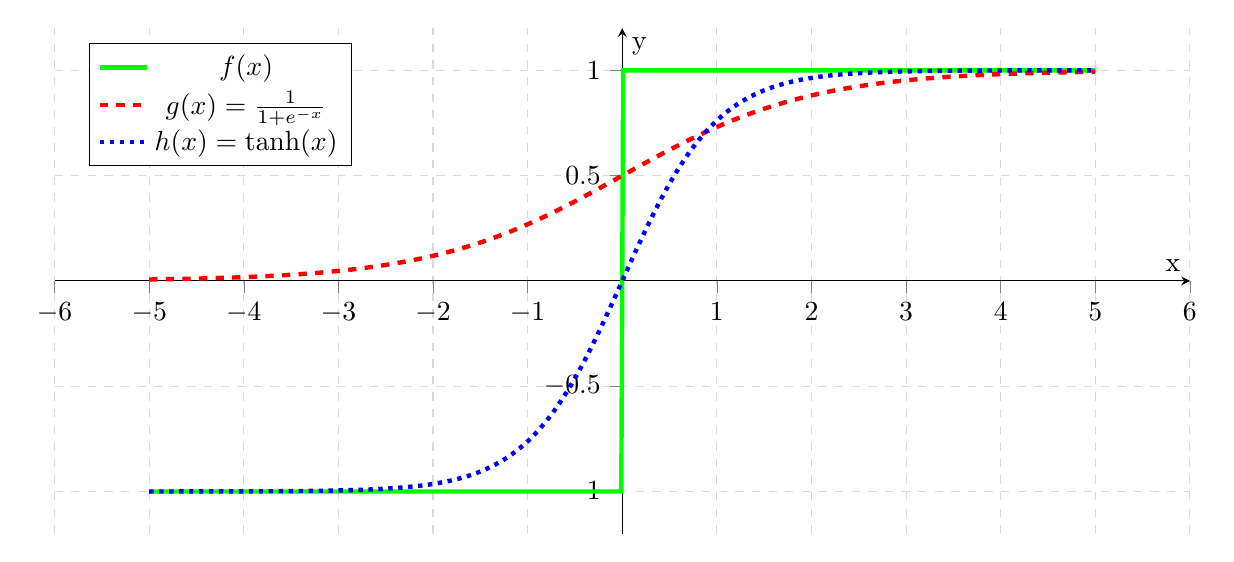
\begin{tikzpicture}[scale=1.0]
        \begin{axis}[
            legend pos=north west,
            axis x line=middle,
            axis y line=middle,
            grid = major,
            width=16cm,
            height=8cm,
            grid style={dashed, gray!30},
            xmin=-5,     % start the diagram at this x-coordinate
            xmax= 5,    % end   the diagram at this x-coordinate
            ymin=-1,     % start the diagram at this y-coordinate
            ymax= 1,   % end   the diagram at this y-coordinate
            %axis background/.style={fill=white},
            xlabel=x,
            ylabel=y,
            tick align=outside,
            enlargelimits=true]
          \addplot[domain=-5:5, green, ultra thick,samples=500] {x < 0 ? -1 : 1};
          \addplot[domain=-5:5, red, ultra thick,samples=500, dashed] {1/(1+exp(-x))};
          \addplot[domain=-5:5, blue, ultra thick,samples=500, dotted] {tanh(x)};
          \addlegendentry{$f(x)$}
          \addlegendentry{$g(x)=\frac{1}{1+e^{-x}}$}
          \addlegendentry{$h(x)=\tanh(x)$}
        \end{axis} 
    \end{tikzpicture}
    \caption{A variation of the sign function $f$ with $f(0) = -1$, the sigmoid function $g$ and the hyperbolic tangend $h$.}
    \label{fig:logistic-function}
\end{figure}

\subsection{Unit step function}\label{f:unitstep}
Not so good, because it's not differentiable. Therefore, the backpropagation
algorithm cannot be used.

\subsection{Sigmoid function}\label{f:sigmoid}
Is great because it is infinitely often differentiable.


\subsection{Hyperbolic tangent}\label{f:tanh}
Also differentiable, but gradient descent converges faster (sometimes?)

\subsection{Softmax}\label{f:softmax}

\[\varphi(a_j) = \frac{e^{a_j}}{\sum_k e^{a_k}}\]
